%%%%%%%%%%%%%%%%%%%%%%%%%%%%%%%%%%%%

\section{Paired data}

%%%%%%%%%%%%%%%%%%%%%%%%%%%%%%%%%%%

\subsection{Paired observations}

\begin{frame}

\dq{200 observations were randomly sampled from the High School and Beyond survey. The same students took a reading and writing test and their scores are shown below. At a first glance, does there appear to be a difference between the average reading and writing test score?}

\begin{center}
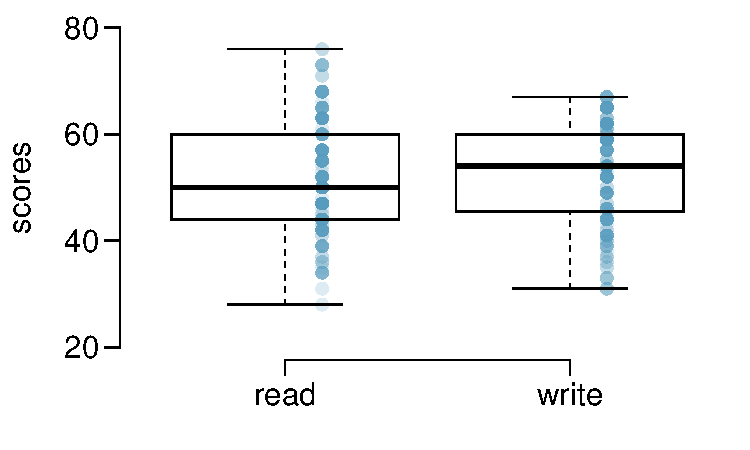
\includegraphics[width=0.5\textwidth]{7-2_paired/figures/hsb2/hsb2_read_write_box}
\end{center}

\end{frame}

%%%%%%%%%%%%%%%%%%%%%%%%%%%%%%%%%%%%

\begin{frame}

\pq{The same students took a reading and writing test and their scores are shown below. Are the reading and writing scores of each student independent of each other?}

{\small
\begin{center}
\begin{tabular}{rrrr}
  \hline
 & id & read & write \\ 
  \hline
1 & 70 & 57 & 52 \\ 
  2 & 86 & 44 & 33 \\ 
  3 & 141 & 63 & 44 \\ 
  4 & 172 & 47 & 52 \\ 
  $\vdots$ &   $\vdots$  &   $\vdots$ &   $\vdots$  \\
  200 & 137 & 63 & 65 \\ 
   \hline
\end{tabular}
\end{center}
}

\begin{multicols}{2}
\begin{enumerate}[(a)]
\item Yes
\solnMult{No}
\end{enumerate}
\end{multicols}

\end{frame}

%%%%%%%%%%%%%%%%%%%%%%%%%%%%%%%%%%%%

\begin{frame}
\frametitle{Analyzing paired data}

\begin{itemize}

\item When two sets of observations have this special correspondence (not independent), they are said to be \hl{paired}.

\pause

\item To analyze paired data, it is often useful to look at the difference in outcomes of each pair of observations. 
\[ \text{diff} = \text{read} - \text{write} \]

\pause

\item It is important that we always subtract using a consistent order.

\end{itemize}

\twocol{0.5}{0.5}{
{\small
\begin{center}
\begin{tabular}{rrrr >{\columncolor[gray]{.9}}r}
  \hline
 & id & read & write & diff \\ 
  \hline
1 & 70 & 57 & 52 & 5 \\ 
  2 & 86 & 44 & 33 & 11 \\ 
  3 & 141 & 63 & 44 & 19 \\ 
  4 & 172 & 47 & 52 & -5 \\ 
  $\vdots$ &   $\vdots$  &   $\vdots$ &   $\vdots$ &   $\vdots$ \\
  200 & 137 & 63 & 65 & -2 \\ 
   \hline
\end{tabular}
\end{center}
}
}
{
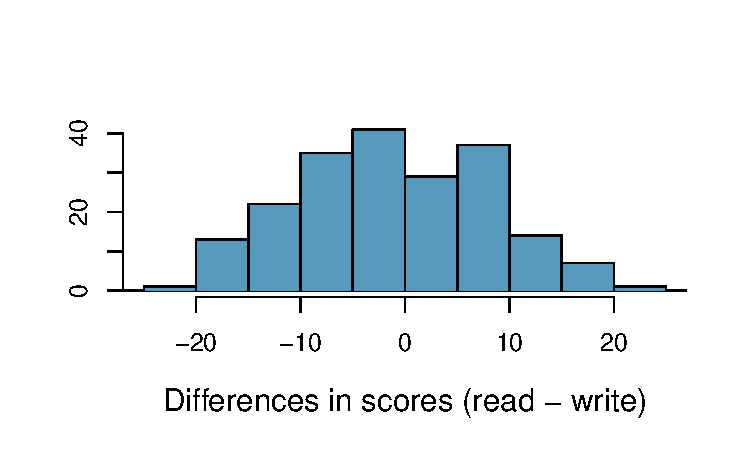
\includegraphics[width=\textwidth]{7-2_paired/figures/hsb2/hsb2_diff_hist}
}

\end{frame}

%%%%%%%%%%%%%%%%%%%%%%%%%%%%%%%%%%%%

\begin{frame}
\frametitle{Parameter and point estimate}

\begin{itemize}

\item \hl{Parameter of interest:} Average difference between the reading and writing scores of \orange{all} high school students.
\[ \mu_{diff} \]

$\:$ \\

\pause

\item \hl{Point estimate:} Average difference between the reading and writing scores of \orange{sampled} high school students.
\[ \bar{x}_{diff} \]

\end{itemize}

\end{frame}

%%%%%%%%%%%%%%%%%%%%%%%%%%%%%%%%%%%%

\subsection{Inference for paired data}

\begin{frame}
\frametitle{Setting the hypotheses}

\dq{If in fact there was no difference between the scores on the reading and writing exams, what would you expect the average difference to be?}

\pause

\soln{0}

$\:$ \\

\pause

\dq{What are the hypotheses for testing if there is a difference between the average reading and writing scores?}

\pause

\begin{itemize}
\item[$H_0$:] There is no difference between the average reading and writing score. 
\[ \mu_{diff} = 0 \]
\item[$H_A$:] There is a difference between the average reading and writing score. 
\[ \mu_{diff} \ne 0 \]
\end{itemize}

\end{frame}

%%%%%%%%%%%%%%%%%%%%%%%%%%%%%%%%%%%%

\begin{frame}
\frametitle{Nothing new here}

\begin{itemize}

\item The analysis is no different than what we have done before.

\item We have data from \orange{one} sample: differences. 

\item We are testing to see if the average difference is different than 0.

\end{itemize}

\end{frame}

%%%%%%%%%%%%%%%%%%%%%%%%%%%%%%%%%%%%

\begin{frame}
\frametitle{Checking assumptions \& conditions}

\pq{Which of the following is true?}

\begin{enumerate}[(a)]
\solnMult{Since students are sampled randomly and are less than 10\% of all high school students, we can assume that the difference between the reading and writing scores of one student in the sample is independent of another.}
\item The distribution of differences is bimodal, therefore we cannot continue with the hypothesis test.
\item In order for differences to be random we should have sampled with replacement.
\item Since students are sampled randomly and are less than 10\% all students, we can assume that the sampling distribution of the average difference will be nearly normal.
\end{enumerate}

\end{frame}

%%%%%%%%%%%%%%%%%%%%%%%%%%%%%%%%%%%

\begin{frame}[shrink]
\frametitle{Calculating the test-statistic and the p-value}

\dq{The observed average difference between the two scores is -0.545 points and the standard deviation of the difference is 8.887 points. Do these data provide convincing evidence of a difference between the average scores on the two exams? Use $\alpha = 0.05$.}

\twocol{0.5}{0.5}
{
\begin{center}
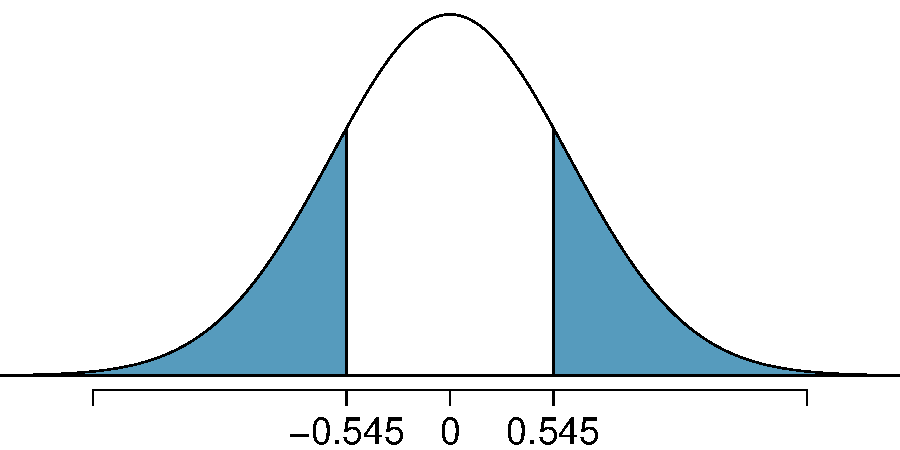
\includegraphics[width=\textwidth]{7-2_paired/figures/hsb2/hsb2_read_write_pval}
\end{center}
}
{
\pause
\begin{eqnarray*}
T &=& \frac{-0.545 - 0}{\frac{8.887}{\sqrt{200}}} \\
&=& \frac{-0.545}{0.628} = -0.87 \\
df &=& 200 - 1 = 199 \\
\pause
p-value &=& 0.1927 \times 2 = 0.3854
\end{eqnarray*}
}
\pause 
$\:$ \\
Since p-value $>$ 0.05, fail to reject, the data do \underline{not} provide convincing evidence of a difference between the average reading and writing scores.

\end{frame}

%%%%%%%%%%%%%%%%%%%%%%%%%%%%%%%%%%%

\begin{frame}
\frametitle{Interpretation of p-value}

\pq{Which of the following is the correct interpretation of the p-value?}

\begin{enumerate}[(a)]
\item Probability that the average scores on the reading and writing exams are equal.
\item Probability that the average scores on the reading and writing exams are different.
\solnMult{Probability of obtaining a random sample of 200 students where the average difference between the reading and writing scores is at least 0.545 (in either direction), if in fact the true average difference between the scores is 0.}
\item Probability of incorrectly rejecting the null hypothesis if in fact the null hypothesis is true.
\end{enumerate}

\end{frame}

%%%%%%%%%%%%%%%%%%%%%%%%%%%%%%%%%%%%

\begin{frame}
\frametitle{HT $\leftrightarrow$ CI}

\pq{Suppose we were to construct a 95\% confidence interval for the average difference between the reading and writing scores. Would you expect this interval to include 0?}

\begin{enumerate}[(a)]
\solnMult{yes}
\item no
\item cannot tell from the information given
\end{enumerate}

\soln{\pause
\begin{eqnarray*} 
-0.545 \pm 1.97 \frac{8.887}{\sqrt{200}} &=& -0.545 \pm 1.97 \times 0.628 \\
&=& -0.545 \pm 1.24 \\
&=& (-1.785, 0.695)
\end{eqnarray*}
}

\end{frame}

%%%%%%%%%%%%%%%%%%%%%%%%%%%%%%%%%%%%